\tikzset{every picture/.style={line width=0.75pt}} %set default line width to 0.75pt

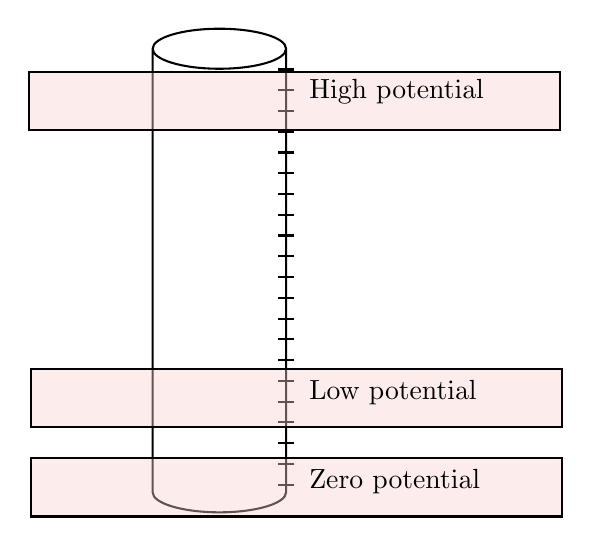
\begin{tikzpicture}[x=0.75pt,y=0.75pt,yscale=-1,xscale=1]
%uncomment if require: \path (0,300); %set diagram left start at 0, and has height of 300

%Shape: Can [id:dp15456700366437115]
    \draw   (164.3,48.84) -- (164.3,262.55) .. controls (164.3,267.88) and (149.91,272.2) .. (132.15,272.2) .. controls (114.39,272.2) and (100,267.88) .. (100,262.55) -- (100,48.84) .. controls (100,43.52) and (114.39,39.2) .. (132.15,39.2) .. controls (149.91,39.2) and (164.3,43.52) .. (164.3,48.84) .. controls (164.3,54.17) and (149.91,58.49) .. (132.15,58.49) .. controls (114.39,58.49) and (100,54.17) .. (100,48.84) ;
%Straight Lines [id:da40290650954202456]
    \draw    (164.3,48.84) -- (164.3,262.55) (168.3,58.84) -- (160.3,58.84)(168.3,68.84) -- (160.3,68.84)(168.3,78.84) -- (160.3,78.84)(168.3,88.84) -- (160.3,88.84)(168.3,98.84) -- (160.3,98.84)(168.3,108.84) -- (160.3,108.84)(168.3,118.84) -- (160.3,118.84)(168.3,128.84) -- (160.3,128.84)(168.3,138.84) -- (160.3,138.84)(168.3,148.84) -- (160.3,148.84)(168.3,158.84) -- (160.3,158.84)(168.3,168.84) -- (160.3,168.84)(168.3,178.84) -- (160.3,178.84)(168.3,188.84) -- (160.3,188.84)(168.3,198.84) -- (160.3,198.84)(168.3,208.84) -- (160.3,208.84)(168.3,218.84) -- (160.3,218.84)(168.3,228.84) -- (160.3,228.84)(168.3,238.84) -- (160.3,238.84)(168.3,248.84) -- (160.3,248.84)(168.3,258.84) -- (160.3,258.84) ;
%Shape: Rectangle [id:dp5549133973023324]
    \draw  [fill={rgb, 255:red, 248; green, 207; blue, 207 }  ,fill opacity=0.4 ] (40.3,60.2) -- (296.3,60.2) -- (296.3,88.2) -- (40.3,88.2) -- cycle ;
%Shape: Rectangle [id:dp8502103142719952]
    \draw  [fill={rgb, 255:red, 248; green, 207; blue, 207 }  ,fill opacity=0.4 ] (41.3,203.2) -- (297.3,203.2) -- (297.3,231.2) -- (41.3,231.2) -- cycle ;
%Shape: Rectangle [id:dp012768010718656964]
    \draw  [fill={rgb, 255:red, 248; green, 207; blue, 207 }  ,fill opacity=0.4 ] (41.3,246.2) -- (297.3,246.2) -- (297.3,274.2) -- (41.3,274.2) -- cycle ;

% Text Node
    \draw (174,62) node [anchor=north west][inner sep=0.75pt]   [align=left] {High potential};
% Text Node
    \draw (174,207) node [anchor=north west][inner sep=0.75pt]   [align=left] {Low potential};
% Text Node
    \draw (174,250) node [anchor=north west][inner sep=0.75pt]   [align=left] {Zero potential};


\end{tikzpicture}